% !TeX root = main.tex
\documentclass{./packages/informe}
\usepackage{./packages/caratula}
\usepackage[T1]{fontenc}
\usepackage[spanish]{babel}
\graphicspath{./files/src/.media/}

\begin{document} 

% caratula 
\titulo{TP 3: Camino mínimo y Flujo máximo}
\subtitulo{}
\fecha{20 de Junio, 2023}
\materia{Algoritmos y Estructuras de Datos III}
% \grupo{Grupo 18}

\integrante{Zaid, Pablo}{869/21}{pablozaid2002@gmail.com}
\integrante{Arienti, Federico}{316/21}{fa.arienti@gmail.com}

\maketitle


% palabras clave y resumen
\addtocontents{toc}{\protect\setcounter{tocdepth}{0}}
\section*{resumen}
\addtocontents{toc}{\protect\setcounter{tocdepth}{3}}
En la teoría de grafos, el problema del \textit{camino mínimo}\footnote{ Ver Thomas H. Cormen; Charles E. Leiserson; Ronald L. Rivest y Clifford Stein. Introduction to algorithms. 2009. Sección 24: \textit{Single-source shortest paths}.\label{foot_1}} se refiere a una serie de problemas relacionados a encontrar, para un grafo ---o digrafo--- \mbox{$G = (V,\ E)$} con función de peso \mbox{$w : E \to \mathbb{R}$} asociada y ciertos pares de vértices $s,\ t \in V$, un conjunto de caminos para los cuales la suma total del peso de sus aristas ---su \textit{distancia}--- es mínima de entre todos los caminos posibles con extremos en algún par $s$ y $t$. En este informe, nos vamos a concentrar en la variante del problema conocida como \textit{camino mínimo a partir de una única fuente}, donde interesa conocer la distancia de cualquier camino mínimo entre una fuente $s \in V$ y todo el resto de los vértices $v \in V \backslash \{s\}$.

Existen diversos métodos para la resolución de este problema. Entre ellos, los algoritmos de \textit{Bellman-Ford} y de \textit{Dijkstra}, que se basan en el concepto de \textit{relajación de aristas}\footnote{ Podemos pensar en el proceso de relajación como un método por el cual se mejora, sucesivamente, la cota superior a la distancia que puede tener un camino mínimo. El mismo se basa en la propiedad de desigualdad triangular: si $\delta : E \to \mathbb{R}$ denota la distancia mínima entre cualquier par de vértices en $V$, entonces para cualquier par de vértices $s$ y $t$ y arista $(u,\ t) \in E$ con $u \neq s$,  $\delta(s,\ t) \leq \delta(s,\ u) + w(u,\ t)$.} para la construcción de una solución.  

El siguiente informe evalúa el problema del \textit{trafico}, explicado en el próximo apartado, y lo reformula como una aplicación particular del problema de \textit{camino mínimo a partir de una única fuente} que aprovecha la propiedad de subestructura óptima de los caminos mínimos. Además, evalúa la eficiencia de la solución propuesta de manera empírica. %en función de la aplicación de diferentes heurísticas. En particular, \textit{union by rank} y \textit{path compression}\footnote{ Ver nota al pie (\ref{foot_1}). Sección 21: \textit{Data Structures for Disjoint Sets}.\label{foot_3}}.

$\\$
\noindent Palabras clave: \textit{camino mínimo, algoritmo de Dijkstra}.

% \newpage

% contenido
\tableofcontents
\newpage

% introduccion
\section{El problema del tráfico}\label{trafico}
% el problema
El problema del \textit{tráfico} que consideraremos tiene la siguiente premisa. Dado una ciudad representada por un conjunto $V$ de $n$ puntos conectados por un conjunto $E$ de $m$ calles unidireccionales, dos puntos críticos $s$ y $t \in V$, y un conjunto
\begin{equation*}
    P := \{p_1 \ ... \ p_k\}    
\end{equation*}
de $k$ calles bidireccionales candidatas, queremos saber cuál es la mínima distancia que deberemos recorrer para llegar de $s$ a $t$, dado que se construya una de estas calles.

Para ello, vamos a contar con la longitud $\ell^c_i$, $1 \leq i \leq m$ de cada calle en la ciudad y la longitud $\ell^p_j$, $1 \leq j \leq k$ de cada calle posible a construir.

Por ejemplo, si tuvieramos la siguiente ciudad ---cuyas calles candidatas están en color gris--- y los puntos críticos $s = 1$ y $t = 4$

\begin{figure}[!htbp]
    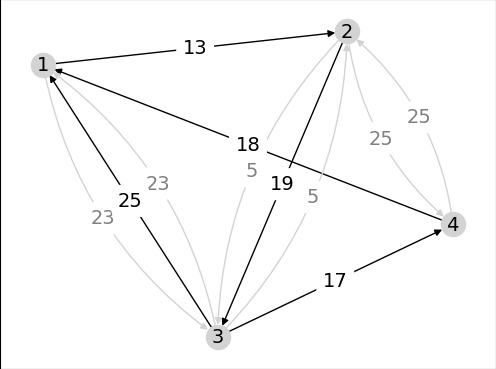
\includegraphics[scale=0.5, trim={0.2cm 0.2cm 0.2cm 0.2cm}, clip]{/files/src/.media/grafo.png} 
    %\caption{s} \label{ejemplo}
\end{figure}
    
\noindent entonces podríamos construir la calle $2 \leftrightarrow 3$ de longitud $5$ para lograr un recorrido mínimo $1 \to 2 \to 3 \to 4$ de largo $35$.

% modelado
\subsection{Modelado como un problema de camino mínimo}\label{modelo} 

A partir del ejemplo anterior, vemos que el problema del \textit{tráfico} se puede modelar de manera intuitiva como un problema de \textit{camino minimo} en grafos: sea $D$ el digrafo asociado a una ciudad $(V,\ E)$ y sea $w: E \to \mathbb{R}_{+}$ una función de peso, donde $w(c_i) = \ell^c_i$, $c_i \in E$ para todo $1 \leq i \leq m$, y $w(p_i) = \ell^p_i$, $p_i \in P$ para todo $1 \leq i \leq k$. Luego, podemos resolver el problema del \textit{tráfico} si evaluamos el mínimo entre todos los caminos mínimos entre $s$ y $t$ para cada digrafo en la sucesión
\begin{equation}\label{eq_1}
    \{D\} \cup \{(V,\ E \cup \{e,\ \bar{e}\}) : e \in P\}
\end{equation}
utilizando la función de peso $w$.

Sin embargo, esto no es eficiente. De emplear el algoritmo de \textit{Dijkstra} con \textit{min-heap}, la complejidad de peor caso estaría en $O(k\cdot m\log n)$. Vamos a ver cómo lo podemos mejorar. 

% algoritmo
\subsection{El algoritmo}

Notar primero que el camino mínimo entre dos vértices $s$ y $t$ satisface la propiedad de \textit{subestructura óptima}\footnote{Ver Cita \ref{foot_1}, sección 16.2: \textit{Elements of a greedy strategy}.}. Esto es, cada sección del camino forma, a su vez, un camino mínimo\footnote{Si no, podríamos reemplazar esta sección por otra de menor distancia, lo que es una contradicción.}. 

Sigue que, si $\delta_D : E \to \mathbb{R}$ es la distancia mínima entre cualquier par de vértices en un digrafo $D = (V,\ E)$ con función de peso $w: E \to \mathbb{R}$ que no tiene ciclos negativos, entonces para cualquier par de vértices $s$ y $t$ en $V$, para los cuales existe un camino $s \rightsquigarrow t$, y una arista $(u,\ v)$ perteneciente a este camino, $\delta_D(s,\ t) = \delta_D(s,\ u) + w(u,\ v) + \delta_D(v,\ t)$.

Vamos a demostrar en la siguiente sección que una consecuencia de esta observación es que, de agregar una arista $e = (u,\ v)$ a $D$ con peso $\ell$ no negativo, entonces 
\begin{equation}\label{eq_2}
    \delta_{D + e}(s,\ t) = \min\{\delta_{D}(s,\ u) + \ell + \delta_{D}(v,\ t),\ \delta_{D}(s,\ t)\}.
\end{equation}

En particular, dado que $\delta_D(s,\ t) = \delta_{D^t}(t,\ s)$\footnote{ Notar que los caminos en un digrafo son \textit{dirigidos}. Luego, las distancias son simétricas respecto al digrafo transpuesto.} y que nuestro problema se restringe a pesos no negativos, estas observaciones nos permiten considerar el siguiente algoritmo.

\lstinputlisting[mathescape=true, language=pseudo, label=trafico, caption={Pseudocódigo para el problema del \textit{tráfico}.}]{files/src/.code/trafico.pseudo}

El mismo aplica un algoritmo de \textit{camino mínimo con única fuente} sobre el grafo de entrada $D$, a partir de $s$, y sobre el grafo transpuesto $D^t$, a partir de $t$, para saber la distancia mínima ---que se guarda en los diccionarios $\delta^s$ y $\delta^t$--- de ambos vértices a todo el resto de los vértices en el digrafo. Luego, aplica la ecuación \ref{eq_2} para determinar cuál es la distancia mínima entre $s$ y $t$ en cada par de digrafos $(D + e,\ D + \bar{e})$\footnote{Esto es equivalente a considerar el digrafo $D + \{e,\ \bar{e}\}$, ya que ambas aristas no pueden pertenecer a un mismo camino mínimo. Esto se debe a que, si ambas aristas pertenecieran en simultáneo, formarían un ciclo.} para cada calle bidireccional $e$ en $P$.

% correctitud
\subsection{Demostración de correctitud}\label{correctitud}  

Dada la discusión anterior, basta demostrar que la ecuación \ref{eq_2} se satisface para demostrar que el algoritmo \ref{trafico} encuentra la distancia del camino mínimo entre $s$ y $t$ dentro del conjunto de digrafos definido por la ecuación \ref{eq_1}.

\begin{proof} 
    Sea $D$ un digrafo $D = (V,\ E)$ con función de peso $w: E \to \mathbb{R}$ que no tiene ciclos negativos y sea  $\delta_G : E \to \mathbb{R}$ la distancia mínima entre cualquier par de vértices en un digrafo $G$ cualquiera.

    Consideremos el digrafo $D+e$, con $e = (u,\ v)$, tal que $e$ es una arista entre dos vértices de $V$ que no está en $D$ y tiene peso $\ell$ no negativo. 
    
    Si $e$ no pertenece a ningún camino mínimo de $s$ a $t$ en $D + e$, sigue trivialmente que $\delta_{D + e}(s,\ t) = \delta_{D}(s,\ t)$, ya que $D \subset D + e$. Si, en cambio, sí pertenece, entonces debe ser que
    \begin{equation*}
        \delta_{D + e}(s,\ t) \leq \delta_{D}(s,\ t)
    \end{equation*} 
    ya que, o bien $e$ \textit{mejora} el camino mínimo entre ambos vértices, o bien lo mantiene igual, pero no puede suceder que lo empeore. Si no, dado que cualquier camino mínimo en $D$ está en $D + e$, el camino que contiene a $e$ no sería mínimo. 
    
    Del resultado anterior, y por la propiedad de \textit{subestructura óptima} del camino mínimo, sigue que
    \begin{equation}\label{eq_3}
        \delta_{D + e}(s,\ t) = \begin{cases}
            \delta_{D + e}(s,\ u) + \ell + \delta_{D + e}(v,\ t) &\text{si}\ e \in\ C_{st}(D+e)\\
            \delta_{D}(s,\ t) &\text{si no}
        \end{cases}
    \end{equation}
    donde $C_{st} \subset D + e$ es el subgrafo de caminos mínimos entre $s$ y $t$.

    Dado que cualquier camino mínimo de $s$ a $u$ y cualquier camino mínimo de $v$ a $t$ en $D + e$ no puede contener a la arista $e$ ---ya que, si no, se formaría un ciclo---, podemos concluir que $ \delta_{D + e}(s,\ u) = \delta_{D}(s,\ u) $ y $ \delta_{D + e}(v,\ t) = \delta_{D}(v,\ t)$. En particular, sigue que la ecuación \ref{eq_3}, es equivalente a
    \begin{equation*}
        \delta_{D + e}(s,\ t) = \min\{\delta_{D}(s,\ u) + \ell + \delta_{D}(v,\ t),\ \delta_{D}(s,\ t)\}.
    \end{equation*}
\end{proof}
    
% complejidad
\subsection{Complejidad temporal y espacial}

El algoritmo \texttt{trafico} depende casi exclusivamente de la implementación de \textit{camino mínimo} que utilicemos. %Considerando que puede haber diferentes valores para los pesos de las aristas no podemos hacer BFS, y como no se sabe si en el grafo hay ciclos, tampoco se puede usar el algoritmo de orden topológico. Estos dos resultan eficientes si se garantizan sus respectivas precondiciones. 
Dado que no tenemos garantias sobre la estructura del grafo de entrada\footnote{En particular, las longitudes pueden ser distintas ---lo que descarta el uso de \textit{BFS}--- y el digrafo no es necesariamente acíclico ---lo que descarta el uso del algoritmo de orden topológico---.}, más allá de que el peso de las aristas es no negativo, la mejor\footnote{ En base a los algoritmos conocidos.} complejidad que podemos lograr corresponde a utilizar el algoritmo de \textit{Dijkstra} sobre una estructura de \textit{fibonacci-heap}. El costo temporal resultante es $\Theta(k + m + n\log n)$, correspondiente a la construcción del digrafo de entrada y su transpuesta, dos invocaciones de \textit{Dijkstra} y las $k$ iteración del ciclo que comienza en la línea $5$ del algortimo \ref{trafico}. Por su parte, el costo espacial es $\Theta(m + n)$, correspondiente a las estructuras de los digrafos y el costo espacial de \textit{camino mínimo}.  %cuyo costo espacial es $\Theta(n)$ y cuyo costo temporal es $\Theta(m + n\log n)$\footnote{Ver cita \ref{foot_1}, sección 24.3.}. Luego, nuestro problema resultaría en una complejidad temporal en $\Theta(k + m + n\log n)$, correspondiente a la construcción del digrafo de entrada y su transpuesta, dos invocaciones de \textit{camino mínimo} y las $k$ iteración del ciclo que comienza en la línea $5$. El costo espacial estaría en $\Theta(m + n)$, correspondiente a las estructuras de los digrafos y el costo espacial de \textit{camino mínimo}. 

%\newpage

% resultados
%\vspace{2em}
\section{Evaluación empírica}
Para revisar la diferencia en eficiencia entre distintas implementaciones de \texttt{trafico}, consideramos las siguientes versiones del algoritmo de \textit{Dijkstra}: 1. sobre un \textit{min-heap}, por un costo temporal en $\Theta(m\log n)$\footnote{Ver cita \ref{foot_1}, sección 24.3.}; 2. utilizando un arreglo de manera \textit{ingenua} ---lo que permite actualizar la distancia a un vértice en tiempo constante, a cambio de un costo en $\Theta(n)$ para encontrar la próxima arista candidata--- con complejidad $\Theta(n^2)$; y 3. utilizando un \textit{queue}\footnote{En este caso, la estructura utilizada es la \textit{priority queue} de C$++$.} ``lazy'' ---en vez de agregar todos los nodos a la cola, estos se van colocando a medida que aparecen en la lista de adyacencia de los nodos candidatos y nunca se remueven---, por una complejidad temporal en $\Theta(m\log n)$.
% Para revisar la diferencia en eficiencia entre distintas implementaciones de \texttt{trafico} sobre el algoritmo de Djikstra consideramos tres algoritmos para solucionar este problema. El primero, al que llamaremos \textit{heap}, utiliza un heap para guardar todas las aristas y luego ir sacando las candidatas. y puede extraer el mínimo en tiempo constante y cambiar una clave en un razonable $\Theta(log(n))$. La complejidad temporal de este algoritmo es $\Theta(mlogn)$\footnote{Ver diapositivas de la clase 7, AED3}. Una segunda implementacion, a la que llamaremos \textit{ingenua}, funciona de la misma manera pero implementa el heap de forma ingenua, con un arreglo de costos y otro de valores. Esto permite cambiar claves en tiempo constante, pero a cambio encontrar el mínimo se hace en $Theta(n)$. La complejidad resultante es $Theta(n^2)$\footnote{Ver diapositivas de la clase 7, AED3}. Finalmente usamos \textit{queue}, una implementacion que utiliza la cola de prioridad del \textit{prelude} de C$++$ y un arreglo \textit{marcados} que indica si un elemento ya pasó por el queue o no. En vez de agregar todos los nodos a la cola como los otros dos algoritmos, este los va colocando en a medida que aparecen en la lista de adyacencia de los nodos candidatos. El arreglo \textit{marcados} evita que se repitan nodos. Tiene complejidad espacial de $Theta(mlogn)$\footnote{Ver diapositivas de la clase práctica 12 sobre camino mínimo}.

Teóricamente, \textit{ingenuo} debería ser más eficiente para instancias \textit{densas}, mientras que los otros dos resultan especialmente buenos para entradas \textit{ralas}. Sin embargo los tres algoritmos tienen distintos detalles de implementación que resultan interesantes de analizar empíricamente.%: Si bien \textit{ingenuo} es asintóticamente superior, realiza mucho trabajo de más al tener que recorrer la estructura entera cada vez para encontrar el mínimo. \textit{Queue} puede recorrer el mismo nodo varias veces si se ingresó a la cola en múltiples instancias, y además no tiene el costo de cambiar claves dentro del heap, pero como queue es una estructura de \textit{prelude} es probable que esté bien optimizada, en comparación con \textit{heap} que fue implementada "a mano".

Para cada implementación realizamos una serie de tests para medir el tiempo de ejecución en función del tamaño de la entrada. Primero, evaluamos la influencia de la ``densidad'' del grafo para muestras aleatorias de tamaño $n = 15.000$, donde dejamos variar la cantidad de aristas $m$ en el rango $15.000$ y $112.492.500$ (caso completo) de a deciles. Luego, con muestras de tamaño $n = 10^4k$ y $m = 2n$, para cada $k$ natural en el rango $1 \leq k \leq 10$ ---para evaluar el desempeño en grafos \textit{ralos}--- y, finalmente, con muestras de tamaño $N = 10^6k$ para cada $k$ natural en el rango $1 \leq k \leq 10$, con $m = 2n$ ---para comparar, en mayor profundidad, el desempeño en grafos ralos de las implementaciones \textit{heap} y \textit{queue}---.

%Para ver empíricamente la diferencia en eficiencia entre estas tres implementaciones, realizamos una serie de evaluaciones, para cada una de estas implementaciones, respecto al tiempo de ejecución en función del tamaño de la entrada. Primero, evaluamos la influencia de la ``densidad'' del grafo para muestras aleatorias de tamaño $n = 15000$ $m = 15000 + 11247750 * k$ para cada $k$ natural  en el rango $1 \leq k \leq 10$, para cómo afecta la cantidad de aristas al tiempo de ejecución en cada algoritmo, luego con muestras de tamaño $N = 10000k$ para cada $k$ natural en el rango $1 \leq k \leq 10$, para observar el desempeño en grafos ralos. Y finalmente con muestras de tamaño $N = 1000000k$ para cada $k$ natural en el rango $1 \leq k \leq 10$, para comparar el desempeño en grafos ralos de \textit{heap} y \textit{queue}.

Efectuamos las primeras dos evaluaciones diez veces para reducir la variación de los resultados y tomamos el promedio aritmético. Para la segunda evaluación lo hicimos $100$ veces, dado que los tiempos eran muy cortos.

Dado que solo nos interesa evaluar distintas implementaciones de \textit{dijkstra}, controlamos los parámetros de la función de la siguiente forma: elegimos $k = 0$, $s = 1$, $t = 2$ y definimos cada arista $x_i = (a_i,\ b_i,\ w_i)$, para todo $1 \leq  i \leq M$, $0 \leq w_i \leq 1000$ y $1 \leq a_i,\ b_i \leq n$ de manera aleatoria, tal que $a_i \neq b_i$ y $(a_i,\ b_i) \neq (a_j,\ b_j)$ para todo $1 \leq i,\ j \leq m$ e $i \neq j$.

%Notar que ninguna de estas decisiones afecta a la complejidad de las implementaciones de Djikstra. En efecto, el valor de K solo es relevante luego de haber corrido Djikstra, y S y T aleatorios no deberían tener efecto sobre la complejidad asintóticamente.

Las figuras \ref{grafico_1} y \ref{grafico_2} exponen los resultados de la experimentación. Los tres algoritmos parecen ---empíricamente--- mantener la misma complejidad, pero con distintas constantes asociadas. Nótese que, a pesar de su superioridad asintótica, \textit{ingenuo} resulta el más lento, incluso en el caso que ilustra un grafo completo. %Quizás tiene constantes demasiado grandes. Claramente \textit{queue} es la más rápida, quizás por la eficiencia de la implementación de la estructura.

\begin{figure}[!htbp]
    \subfloat{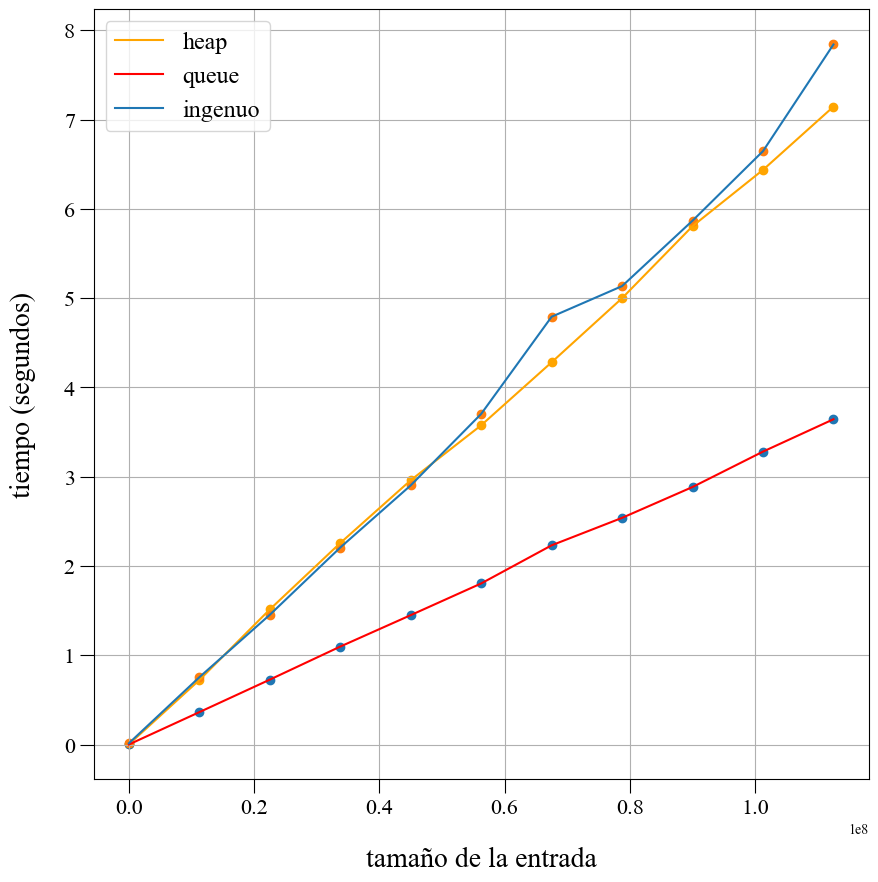
\includegraphics[scale=0.48, clip, trim={0.2cm 0 0 0}]{./files/src/.media/comparacion_triple.png}}

    \caption{Tiempo de ejecución de \texttt{trafico} en función del porcentaje de ``densidad'' del grafo de entrada, con $n = 15.000$, para las implementaciones \textit{ingenuo}, \textit{heap}, y \textit{queue}.}
    \label{grafico_1}
% \end{figure}

% % %\vspace{0.5em}
% \begin{figure}[!htbp]
    \subfloat{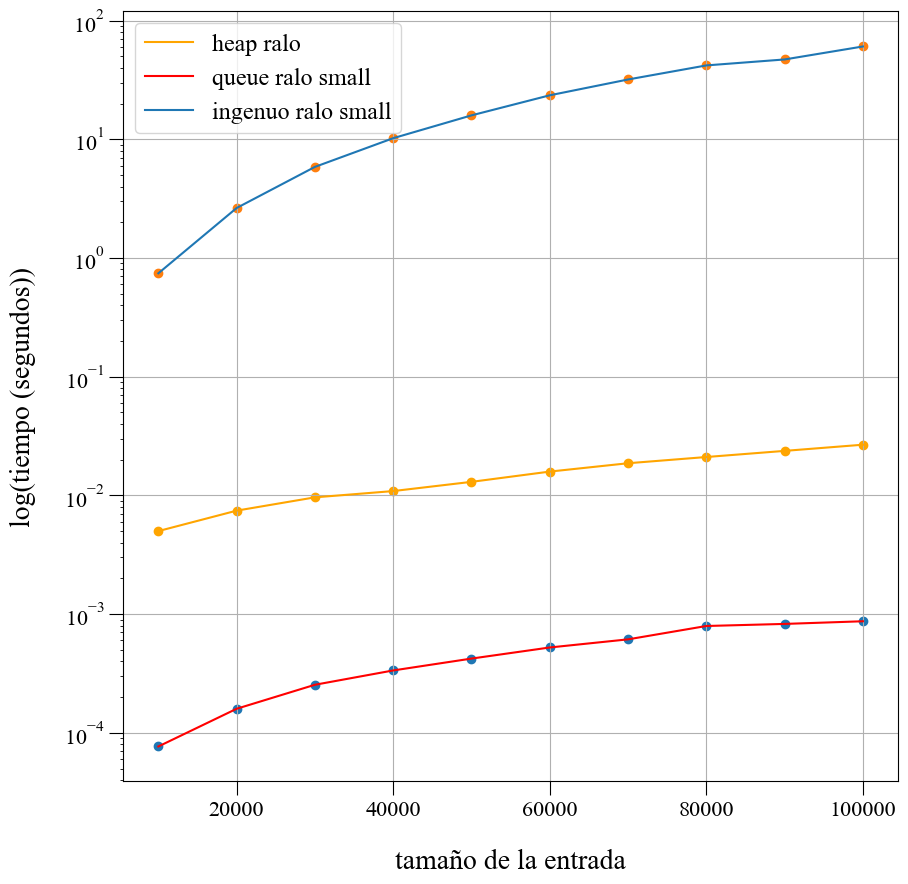
\includegraphics[scale=0.48, clip]{./files/src/.media/comparacion_rala_small.png}}
    %\hfill
    $\ \ \ \ $
    \subfloat{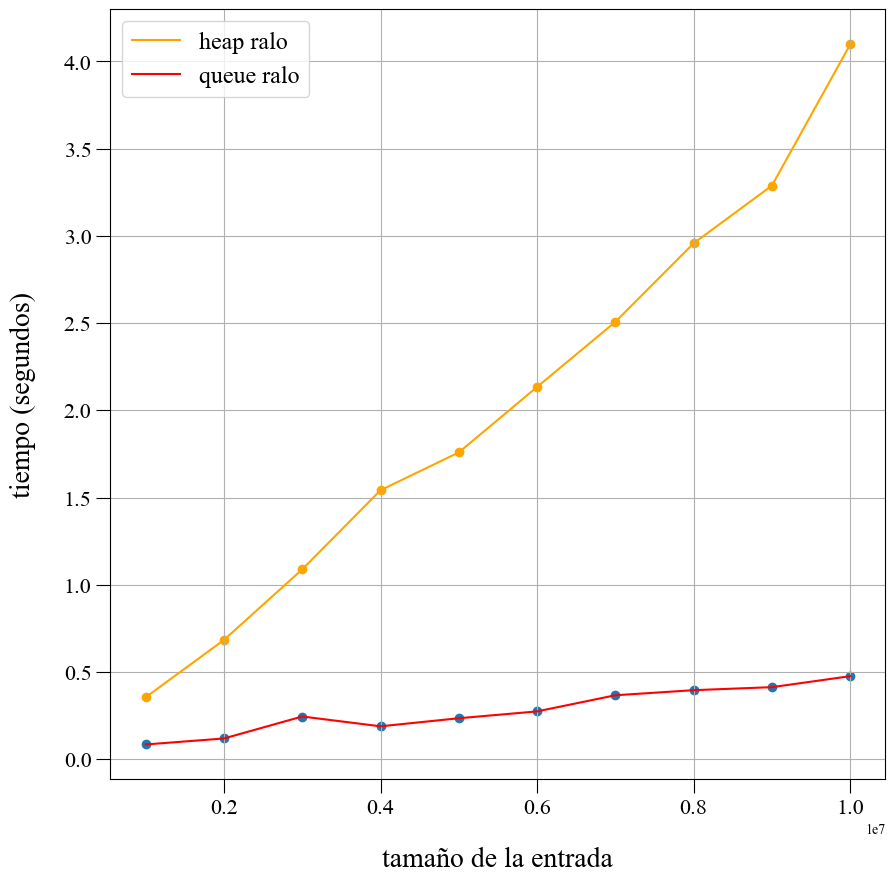
\includegraphics[scale=0.48, clip]{./files/src/.media/comparacion_rala_doble.png}}

    \caption{Izquierda: tiempo de ejecución (log) en función del tamaño de entrada $n$ para los algoritmos \textit{ingenuo}, \textit{heap}, y \textit{queue}. Derecha: tiempo de ejecución en función del tamaño de entrada $n$, con valores grandes, para \textit{heap} y \textit{queue}.}
    \label{grafico_2}
\end{figure}

Por su parte, es llamativo que \textit{queue} tenga mejor tiempo, ya que puede llegar a recorrer el mismo nodo varias veces si se ingresó a la cola en múltiples instancias. Sin embargo, consideramos que, como la estructura es parte de la biblioteca \textit{prelude} de C$++$, es probable que esté bien optimizada, en comparación con \textit{heap} que fue implementada ``a mano''.

%La figura \ref{grafico_2} expone los resultados de las experimentaciones en grafos \textit{ralos}. Notese que el algoritmo \textit{ingenuo} resultó extremadamente ineficiente en esta situación, por lo que se debieron utilizar instancias pequeñas para poder compararlo con los otros algoritmos. Como los tiempos de \textit{heap} y \textit{queue} son demasiado bajos en esta instancia, se comparan los dos solos con una entrada 100 veces más grande. De vuelta se nota una clara diferencia a favor del algoritmo \textit{queue}.
\newpage

% apendice
% \section{Apéndice}
% \input{files/src/apendice.tex}
% \newpage

%bibliografia - requiere que haya citas
% \bibliographystyle{plain}
% \bibliography{./files/citations.bib}
% \newpage

\end{document}
